\documentclass[12pt]{article}
\usepackage[T1]{fontenc}
\usepackage{template/sbc-template}
\usepackage{graphicx,url}
\usepackage[utf8]{inputenc}
\usepackage[brazil]{babel}
\sloppy
\title{Previsão mensal de indicadores agregados de crédito do SCR.data: um estudo piloto com CatBoost e Chronos-2}
\author{João Alves Passos, Túlio Kenji Yoshimura}
\address{Afiliação a confirmar antes da submissão}
\begin{document}
\maketitle
\begin{abstract}
We investigate one-month-ahead forecasts of two aggregate credit ratios using
Brazilian SCR.data monthly snapshots from 2025. The protocol compares temporal
baselines, supervised CatBoost regressors and a pretrained Chronos-2 model.
Calendar joins prevent nonconsecutive targets and features use only past data.
The study separates validation from the December test and reports coverage.
Publication delays, revisions and a single annual cycle limit operational
interpretation and generalization. The naive baseline achieved lower test MAE
for both targets in the common pilot sample.
\end{abstract}
\begin{resumo}
Investigamos previsões de um mês para duas proporções de crédito agregado do
SCR.data de 2025. O protocolo compara baselines temporais, regressores CatBoost
supervisionados e Chronos-2 pré-treinado. Junções por calendário impedem alvos
não consecutivos e os atributos usam somente o passado. A validação é separada
do teste em dezembro e a cobertura é reportada. Atrasos de publicação, revisões
e um único ciclo anual limitam a interpretação operacional e a generalização.
Na amostra comum, o ingênuo obteve menor MAE nos dois alvos.
\end{resumo}
\noindent\textbf{Palavras-chave:} previsão temporal; crédito agregado; SCR.data.
\newline\textbf{Keywords:} time series forecasting; aggregate credit; SCR.data.

\section{Introdução}
Indicadores agregados de crédito permitem acompanhar diferenças entre recortes
econômicos, sem estimar o risco individual de um tomador. O objetivo deste estudo
é prever, para cada perfil observado e elegível, a proporção de inadimplência e
a proporção de ativos problemáticos no mês seguinte. A pergunta experimental é
se modelos supervisionados ou fundacionais melhoram o erro absoluto frente a
referências que repetem ou resumem o passado recente.

O sistema separa leitura, validação, transformação, atributos, modelos e
interpretação textual. Um LLM de briefing pode interpretar métricas calculadas,
mas não participa da geração ou avaliação das previsões.

\section{Dados e unidade de observação}
Utilizamos somente os doze CSVs locais de janeiro a dezembro de 2025,
provenientes do SCR.data, versão 2 \cite{bcb}. Os arquivos originais permanecem
inalterados. O manifesto registra tamanho, SHA256 e data de modificação local;
a data efetiva de extração é desconhecida. A inspeção confirmou separador
ponto e vírgula, vírgula decimal, campos entre aspas e leitura UTF-8. Não se
normalizam grafias, espaços ou categorias silenciosamente.
\IfFileExists{generated/data-summary.tex}{A base contém 3.764.842 observações perfil/mês em 12 meses. Foram identificados 399.480 perfis distintos; somente 236.638 aparecem nos doze meses. As ausências de perfil entre meses reduzem a amostra supervisionada e não representam saldo zero.}{}

A unidade é perfil por mês. A chave contém UF, segmento, cliente,
CNAE/ocupação, porte, modalidade, submodalidade, origem dos recursos e
indexador. As duas últimas dimensões constam do cabeçalho real e evitam
misturar operações com origens ou indexadores distintos. Cada chave é única
no mês; duplicatas ou totais explícitos fazem a ingestão falhar, em vez de
serem somados automaticamente. Não há agregação de níveis diferentes.

Calculam-se os alvos como razões entre os saldos de carteira inadimplente ou
ativo problemático e carteira ativa. Denominador não positivo ou não finito,
numerador negativo, não finito ou superior ao denominador produzem ausente.
Ausências de observação nunca se tornam zero. Categorias especiais como
``Indisponível'' são mantidas. O número de operações, que contém códigos
especiais, não é atributo de treinamento. A auditoria desta execução não
encontrou chaves vazias nem razões inválidas pelas regras implementadas.

A metodologia oficial \cite{bcbmet} informa divulgação após cerca de 30 dias e
possibilidade de substituição de documentos. A partir de janeiro de 2025,
ativos problemáticos correspondem à classificação informada pelas instituições
(característica especial 19). Não reconstruímos os vintages de publicação.
Logo, o experimento usa data-base e o snapshot disponível na extração; simular
acesso imediato ao fechamento pode ser otimista operacionalmente. Os resultados
não representam backtest com disponibilidade real de publicação.

\section{Metodologia e protocolo temporal}
Os rótulos são obtidos por junção exata de perfil e mês calendário seguinte.
Uma observação em fevereiro não recebe abril como alvo se março estiver
ausente. Os atributos incluem perfil, saldos e proporções da origem, mês do
ano, lags de um e dois meses e média de três meses. A média requer três meses
consecutivos válidos. Todas as entradas são determinadas até a origem.

\begin{table}[ht]
\centering
\caption{Divisão por origem e alvo; sem reajuste após a validação.}
\label{tab:protocol}
\begin{tabular}{lll}
\hline
Etapa & Origens em 2025 & Alvos em 2025 \\
\hline
Treino & janeiro--agosto & fevereiro--setembro \\
Validação & setembro--outubro & outubro--novembro \\
Teste & novembro & dezembro \\
\hline
\end{tabular}
\end{table}

O CatBoost é ajustado somente no treino da Tabela~\ref{tab:protocol}. A
validação escolhe a profundidade; o teste não seleciona hiperparâmetros e não
há reajuste com o target de novembro. O histórico de proporções de outubro
ou novembro pode ser usado na respectiva origem como entrada, sob a hipótese
explícita de data-base, sem entrar no ajuste dos pesos. Muitos perfis não
equivalem a muitos períodos independentes. Backtesting adicional e inferência
de incerteza entre origens permanecem pendentes.

\subsection{Baselines e modelos}
O baseline ingênuo usa a proporção da origem, imediatamente anterior ao mês
previsto. A média móvel usa três meses consecutivos. O drift soma ao valor
atual metade da diferença entre ele e o valor de dois meses antes. Métodos
sem histórico suficiente se abstêm. O baseline sazonal de doze meses é
indisponível: prever dezembro de 2025 exigiria dezembro de 2024.

CatBoost \cite{catboost} trata atributos categóricos e relações não lineares.
São dois regressores independentes, permitindo que a ausência de um rótulo
não elimine o outro. A grade contém profundidades 4 e 6; cada candidato usa
200 iterações, taxa 0,05, perda MAE, semente 42 e quatro threads CPU.
Categorias são strings, com marcador de ausência; números ausentes usam
\texttt{nan\_mode=Min}. O menor MAE de validação escolhe cada modelo,
persistido em formato CBM junto à configuração. Trata-se de treinamento
supervisionado nos dados SCR, não de pré-treinamento fundacional.

Chronos-2 \cite{chronos2} é usado sem ajuste de pesos, com checkpoint
\texttt{amazon/chronos-2}, revisão registrada no manifesto. Cada alvo é
previsto separadamente como série univariada, com contexto comum de três meses
consecutivos, horizonte um e mediana preditiva. Não se compartilham séries
entre perfis e não se fornecem covariáveis futuras. A implementação usa
\texttt{chronos-forecasting 2.3.2}. O piloto CPU seleciona perfis cujo SHA256
da chave, serializada em JSON UTF-8, tem resto zero módulo 1024. A seleção é
independente dos saldos e rótulos. A execução integral fica disponível pelo argumento
\texttt{--chronos-sample-modulus 1}; fine-tuning é opcional e não foi realizado.

O contraste de entradas é deliberado: CatBoost recebe perfil e saldos além do
histórico; Chronos recebe apenas três proporções. A comparação mede sistemas
com informações diferentes, não isola o efeito da arquitetura. Perfis novos
podem receber previsão CatBoost com números ausentes; média, drift e Chronos
se abstêm até obter contexto. Categorias novas não são unificadas com antigas.

\subsection{Avaliação e reprodutibilidade}
MAE é a métrica principal, acompanhada de RMSE e $R^2$, por alvo.
As razões estão na escala 0--1; os erros multiplicados por 100 são expressos
em pontos percentuais (pp). $R^2$ fica indefinido para menos de duas amostras
ou alvo constante. Reportam-se número de rótulos válidos, número de previsões,
cobertura e contagem de previsões fora de $[0,1]$. Não se aplica clipping.
Há tabelas por mês, UF, cliente e segmento e uma comparação principal na
interseção dos métodos executados. Fora da interseção, erros com cobertura
diferente devem ser lidos separadamente.
Cada perfil tem peso igual na métrica; não há ponderação por saldo de carteira.

Os intermediários, modelos e previsões são persistidos separadamente.
Manifestos registram períodos, semente, checkpoint, hashes e cobertura.
O exportador gera tabelas e figuras diretamente das métricas calculadas;
os comandos e caminhos estão documentados no repositório. Os testes usam
fixtures sintéticas e substitutos sem rede, que não integram os resultados.

\section{Resultados}
As Tabelas~\ref{tab:results} e~\ref{tab:coverage} distinguem comparação comum
e cobertura total; a Figura~\ref{fig:mae} sintetiza os erros na amostra comum.
\par
\IfFileExists{generated/discussion.tex}{Para ativos problemáticos, o menor MAE foi do método Ingênuo: 3.733 pp em 267 perfis. Para inadimplência, o menor MAE foi do método Ingênuo: 3.822 pp em 267 perfis. A ordenação por MAE em um único mês não demonstra superioridade geral; RMSE e cobertura devem ser considerados conjuntamente.}{}
\par
\IfFileExists{generated/results.tex}{\begin{table}[ht]
\centering
\caption{Teste em dezembro: interseção dos métodos executados, sem clipping.}
\label{tab:results}
\small
\begin{tabular}{llrrrr}
\hline
Alvo & Método & $n$ & MAE (pp) & RMSE (pp) & $R^2$ \\
\hline
Inad. & Ingênuo & 267 & 3.822 & 14.407 & 0.803 \\
Inad. & Média3 & 267 & 4.936 & 15.263 & 0.778 \\
Inad. & Drift3 & 267 & 5.108 & 15.881 & 0.760 \\
Inad. & CatBoost & 267 & 3.863 & 14.280 & 0.806 \\
Inad. & Chronos-2 & 267 & 4.065 & 14.566 & 0.798 \\
Problem. & Ingênuo & 267 & 3.733 & 13.025 & 0.876 \\
Problem. & Média3 & 267 & 5.867 & 15.491 & 0.825 \\
Problem. & Drift3 & 267 & 5.667 & 15.835 & 0.817 \\
Problem. & CatBoost & 267 & 3.861 & 12.980 & 0.877 \\
Problem. & Chronos-2 & 267 & 4.073 & 13.298 & 0.871 \\
\hline
\end{tabular}
\end{table}}{
Resultados numéricos pendentes de exportação de uma execução concluída.
Nenhuma previsão simulada é apresentada como resultado real.}
\IfFileExists{generated/coverage.tex}{\begin{table}[ht]
\centering
\caption{Cobertura no conjunto total de rótulos elegíveis do teste.}
\label{tab:coverage}
\small
\begin{tabular}{llrrr}
\hline
Alvo & Método & Previsões avaliadas & Cobertura (\%) & Fora de [0,1] \\
\hline
Inad. & Ingênuo & 296864 & 100,000 & 0 \\
Inad. & Média3 & 279548 & 94,167 & 0 \\
Inad. & Drift3 & 279548 & 94,167 & 19694 \\
Inad. & Linear & 296864 & 100,000 & 48673 \\
Inad. & Árvore & 296864 & 100,000 & 0 \\
Inad. & k-NN & 296864 & 100,000 & 0 \\
Inad. & CatBoost & 296864 & 100,000 & 92681 \\
Inad. & Chronos-2 & 267 & 0,090 & 17 \\
Problem. & Ingênuo & 296864 & 100,000 & 0 \\
Problem. & Média3 & 279548 & 94,167 & 0 \\
Problem. & Drift3 & 279548 & 94,167 & 23113 \\
Problem. & Linear & 296864 & 100,000 & 36135 \\
Problem. & Árvore & 296864 & 100,000 & 0 \\
Problem. & k-NN & 296864 & 100,000 & 0 \\
Problem. & CatBoost & 296864 & 100,000 & 12138 \\
Problem. & Chronos-2 & 267 & 0,090 & 31 \\
\hline
\end{tabular}
\end{table}}{}
\IfFileExists{generated/test_mae.png}{
\begin{figure}[ht]
\centering
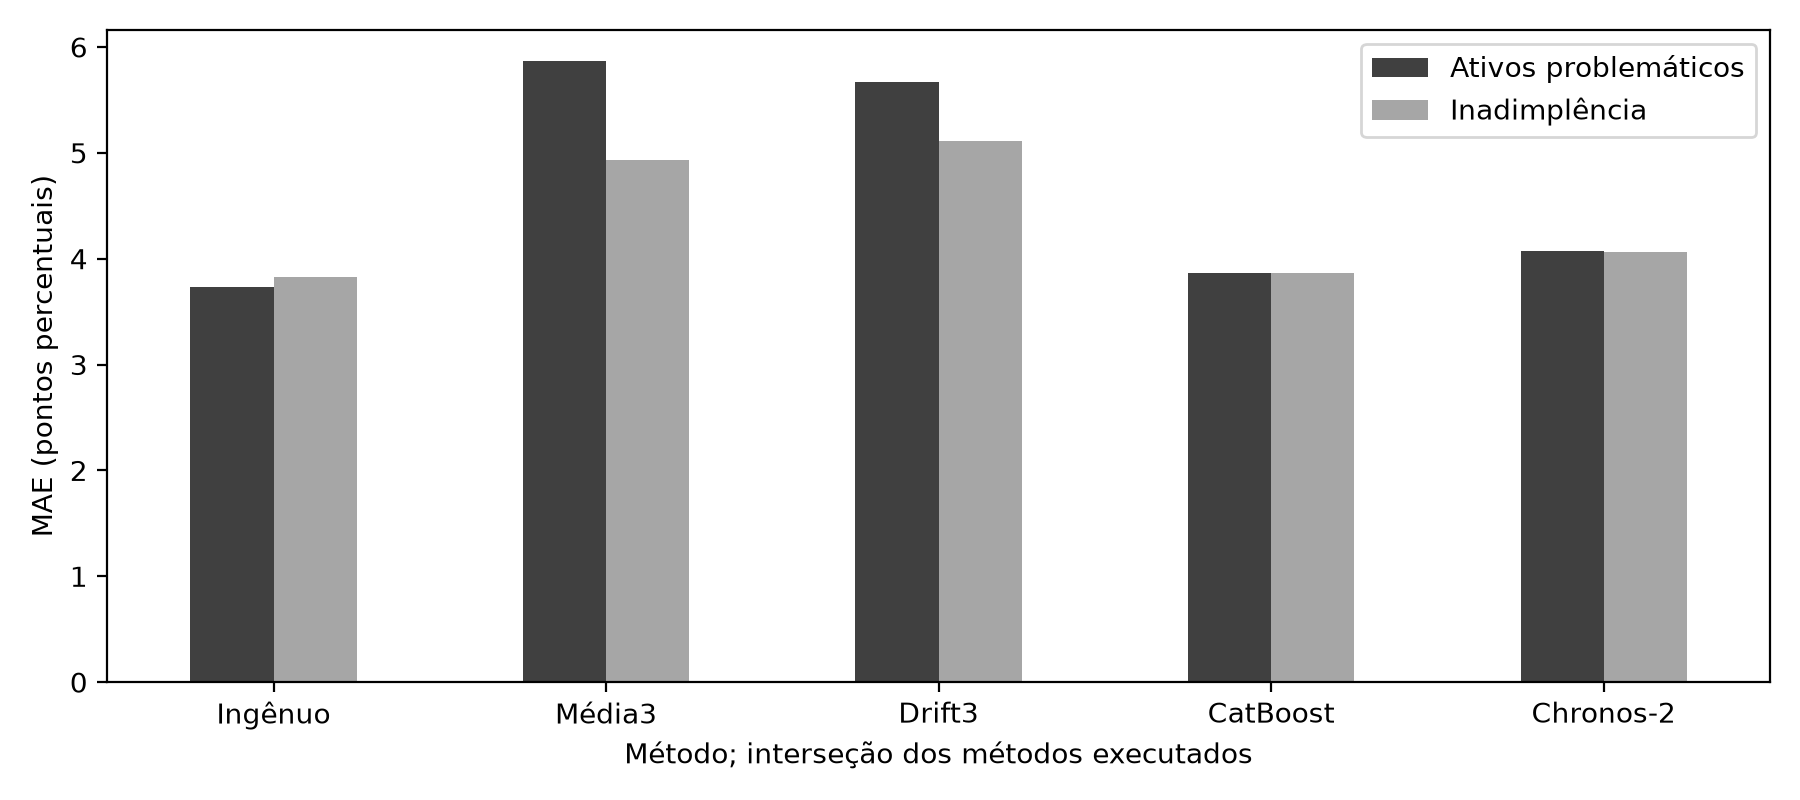
\includegraphics[width=.94\textwidth]{generated/test_mae.png}
\caption{MAE calculado no teste, na interseção dos métodos executados.}
\label{fig:mae}
\end{figure}}{}

As evidências completas de cobertura, configuração e tempo encontram-se nos
arquivos gerados e no relatório de execução em \texttt{docs/}. As métricas
da interseção referem-se ao piloto selecionado para Chronos quando este é
executado, e não à totalidade dos perfis brasileiros. Resultados por grupo
com poucas observações são descritivos e não sustentam rankings estáveis.
Foram usadas 2.415.028 amostras de treino e 591.891 de validação por alvo.
As profundidades escolhidas foram 6 para inadimplência e 4 para ativos
problemáticos. Os quatro ajustes e a predição CatBoost levaram 1.508,7 s;
o piloto Chronos isolado, incluindo leitura preparada, levou 74,6 s.

\section{Discussão e limitações}
Há somente doze meses e um ciclo sazonal, com um único mês de teste.
A diversidade transversal dos perfis não resolve essa limitação temporal.
Amostras pequenas do piloto Chronos restringem a extrapolação. A revisão
do snapshot, o atraso de publicação, mudanças de categoria e perfis ausentes
podem alterar os resultados. Não se verifica causalidade, não se estima risco
individual e não se recomenda decisão automática de concessão de crédito.
O corpus e o corte temporal de pré-treinamento do checkpoint Chronos não foram
auditados em relação ao SCR; não se pode excluir contaminação externa do
benchmark. A ausência de vazamento nas junções locais não resolve esse risco.

Não se instrumentou o pico de memória. O briefing permaneceu desacoplado,
sem chamadas a provedores de texto. Afiliação e limite de páginas do evento
precisam de confirmação antes da submissão.

\section{Conclusão}
O estudo entrega um protocolo auditável para previsão de duas proporções
agregadas, com alinhamento por calendário e separação entre seleção e teste.
A comparação deve ser interpretada como piloto restrito a 2025. A reprodução
com vintages de publicação e mais ciclos temporais, mediante nova autorização
de dados, é necessária antes de alegar generalização operacional robusta.
\bibliographystyle{template/sbc}
\bibliography{references}
\end{document}
